\section{Experiment 3 : Improve Relevance Distribution}
The results from previous experiment are a strong evidence that better structured cell architecture leads to better explanation. However, there are some cases that the purposed architectures fail to distribute relevance properly.  \addfigure{\ref{fig:rel_failed_cases}} shows such cases. \todo{Here ... should not propagate relevances to .... }


Given the motivation above, this experiment aims to extend the proposed architectures further to better address the problem. More precisely, we consider the same classification problem as described in Section \ref{sec:exp2_prob_formulate} and propose 3 improvements, namely stationary dropout, employing gating units,  and literal connections.

\subsection{Proposal 1 :  Stationary Dropout}
Dropout is a simple regularization technique that randomly suspends activity of neurons during training. This randomized suspension allows the neurons to learn more specific representations and reduces chance of overfitting.  It is also directly related to explanation quality. \addfigure{\ref{fig:lenet_various_dropout}} shows explanations of LeNet trained with different dropout probability.

\begin{figure}[!htb]
\centering
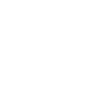
\includegraphics[draft,width=0.5\textwidth]{/sketch/placeholder}
\caption{LeNet with various dropout values} 
\label{fig:lenet_various_dropout}  
\end{figure}

However, unlike typical feedforward architectures, RNN layers are reused across time step, hence a question arises whether the same neurons in those layers should be suspended or they should be different neurons. \addfigure{\ref{fig:lstm_naive_dropout}} and \addfigure{\ref{fig:lstm_variational_dropout}} illustrates these 2 different approaches where different colors represent different dropping activities. In particular, this stationary dropout was first proposed by \cite{GalTheoreticallyGroundedApplication2016} who applied  the technique to LSTM and GRU and found improvements on language modeling tasks.

\begin{figure}[!htb]
\centering
\subfloat[Naive Dropout]{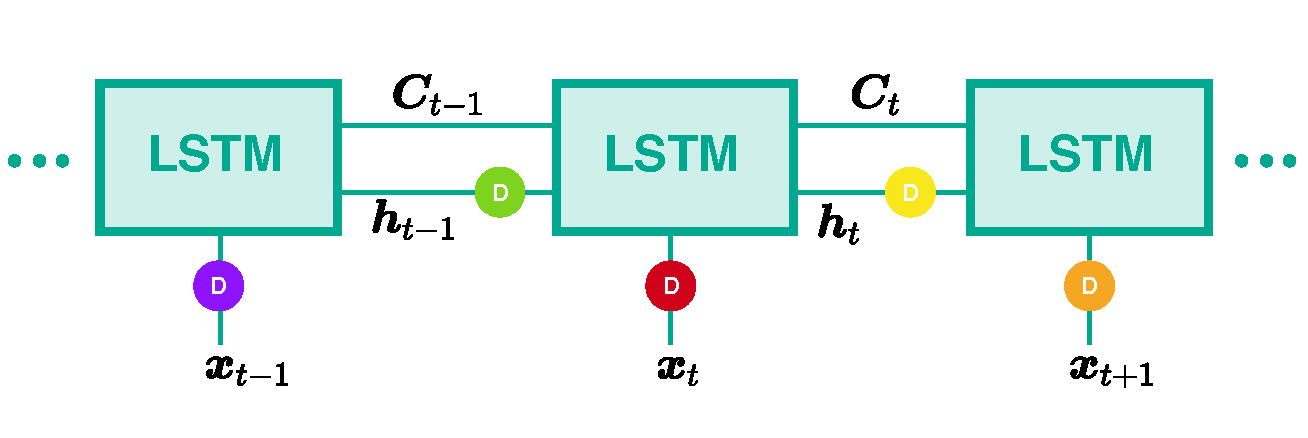
\includegraphics[width=0.8\textwidth]{sketch/lstm_naive_dropout} \label{fig:lstm_naive_dropout}} \\
\subfloat[Stationary Dropout]{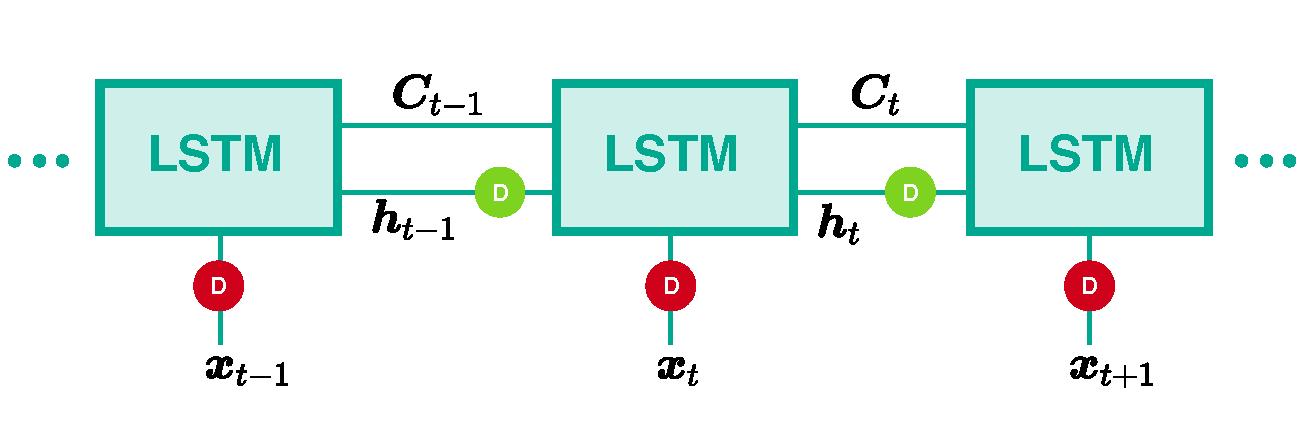
\includegraphics[width=0.8\textwidth]{sketch/lstm_variational_dropout} \label{fig:lstm_variational_dropout}}

\end{figure}

\subsection{Proposal 2 : Gating units}
\begin{figure}[!htb]
\centering
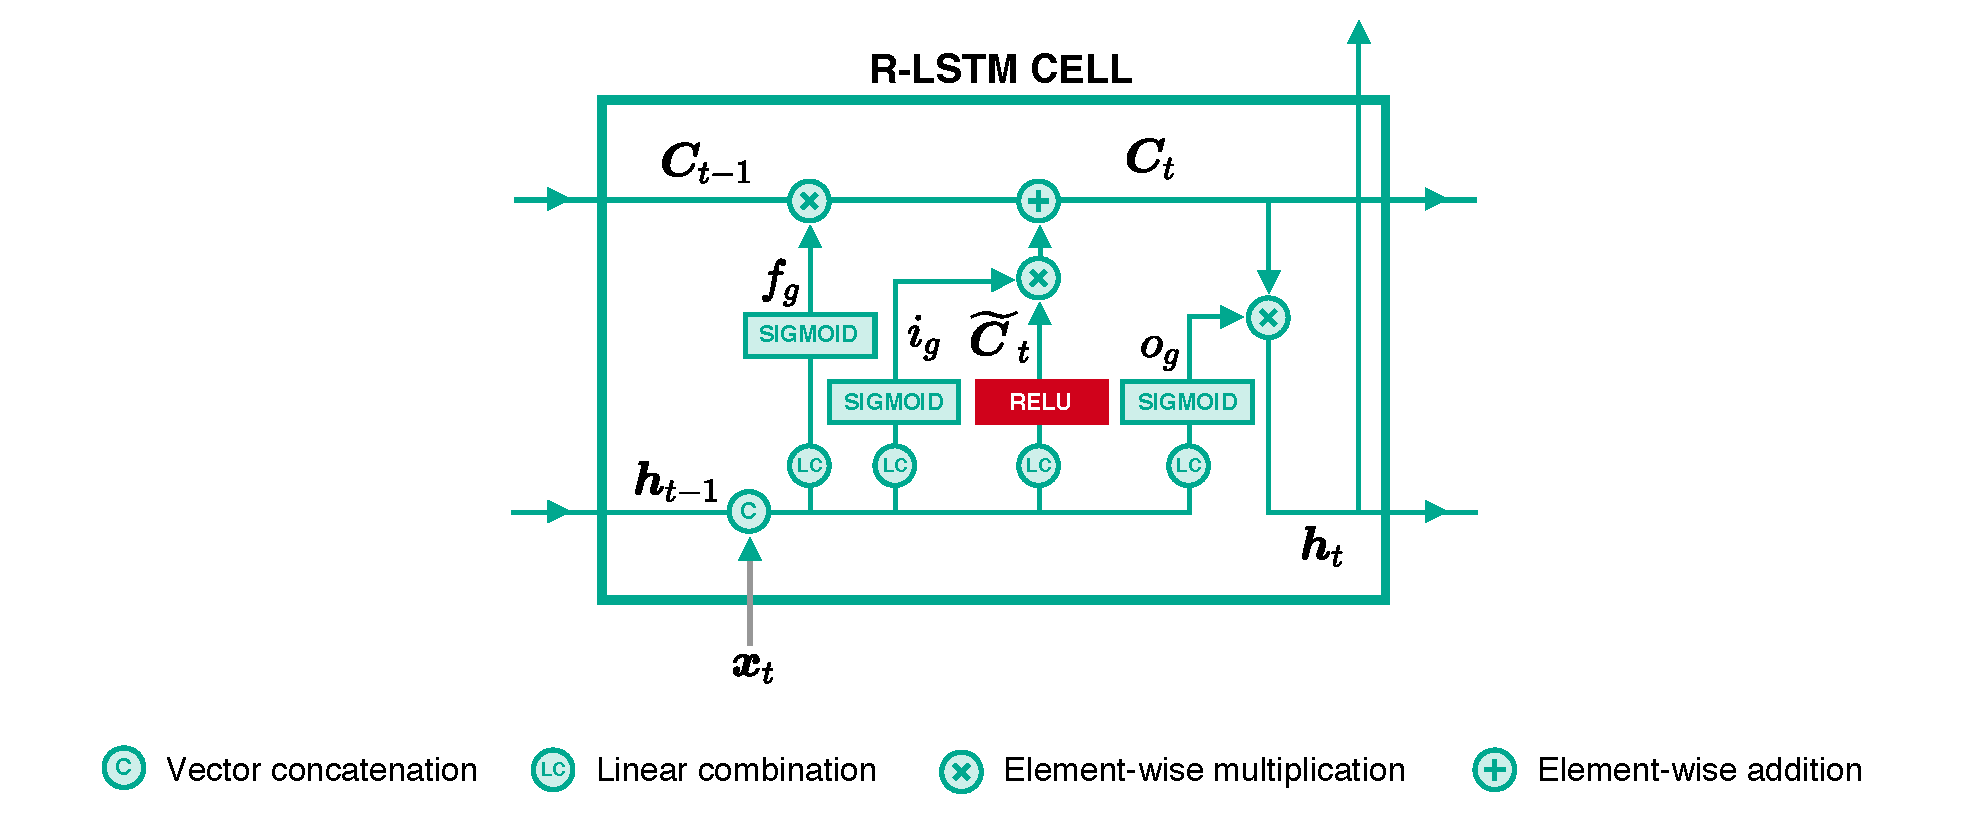
\includegraphics[width=1\textwidth]{sketch/relu_lstm}
\caption{R-LSTM Structure} 

\label{fig:relu_lstm} 
\end{figure}

It is already shown that gating units and addictive updates are critical mechanisms that enable LSTM to learn long term dependencies \cite{GreffLSTMsearchspace2017, Jozefowiczempiricalexplorationrecurrent2015a}. However, LSTM is not readily applicable for methods we are considering in this thesis. More precisely, the use of sigmoid and tanh activations violates the assumption of GB and DTD. Therefore, we propose a slight modified version of LSTM where ReLU activations are used to compute cell state candidates $\widetilde{C}_t$ instead of tanh functions. This results $C_t \in \mathbb{R}^+$, hence the tanh activation for $h_t$  is also removed.  From the following, we will refer this architecture as R-LSTM to differentiate from the original.  \addfigure{\ref{fig:relu_lstm}} presents an overview of R-LSTM architecture.


\subsection{Proposal 3 : Convolutional layer with literal connections}
As discussed in Section \ref{sec:conv}, convolution and pooling operator enable NNs to learn hierarchical representations, which are directly beneficial to explanation quality. The \rnncell{ConvDeep} architecture we proposed in Section \label{sec:rnn_cell} does not seem to exploit this properly because it has recurrent connections only layers after the convolutional and pooling layers. This can be analogically viewed that ConvDeep shares high-level features between step instead of low-level features. This might lead to obscure low-level features in the explanation. \addfigure{\ref{fig:conv_literalconn}} shows the architecture with literal connections are highlighted in red.


 \begin{figure}[!htb]
\centering
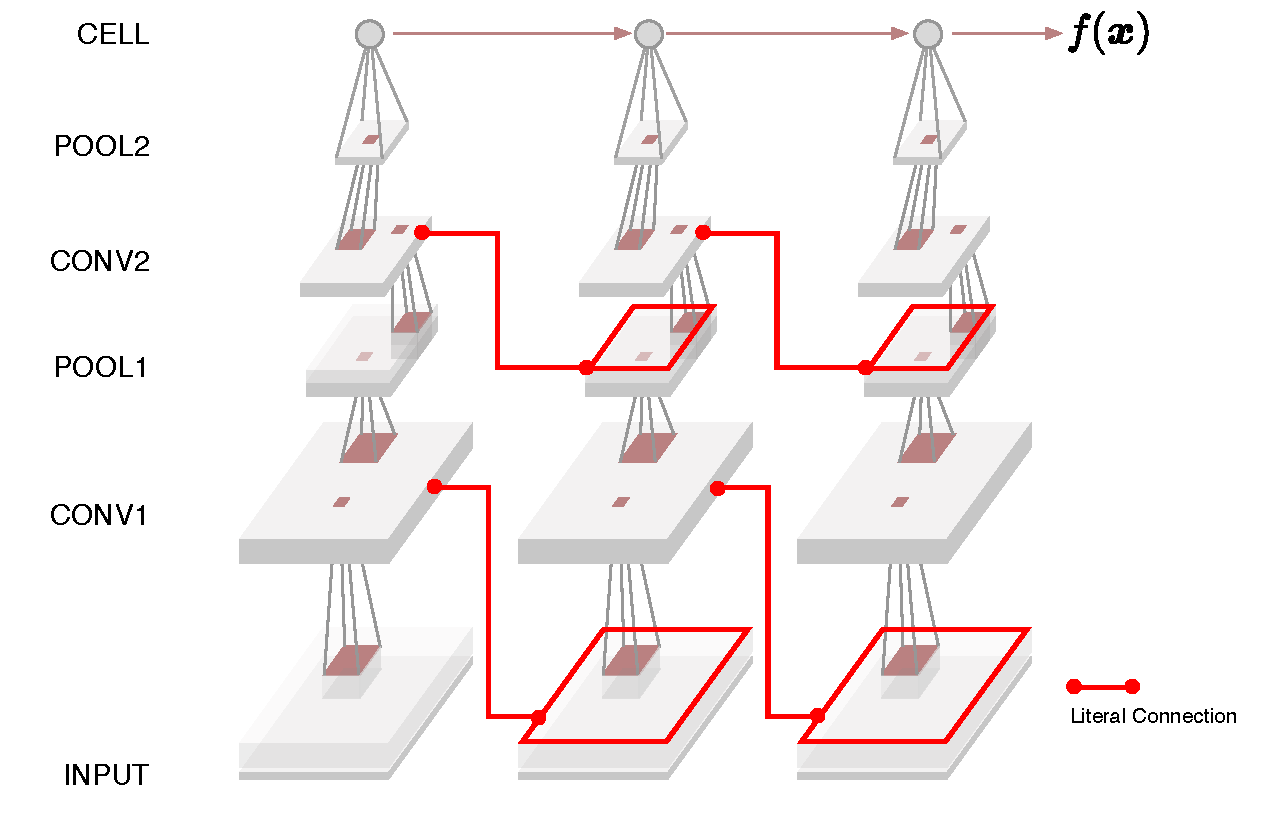
\includegraphics[width=\textwidth]{sketch/conv_literalconn}
\caption{ConvDeep with literal connections(\rnncell{Conv$^+$Deep})} 
\label{fig:conv_literalconn}
\end{figure}

Therefore, we propose an extension of ConvDeep architecture where result of convolution operator is also incorporated into the operator in the next step. We name this connection as \textit{literal connection} and refer \rnncell{Conv$^+$Deep} to this proposed architecture. 

%\subsection{Setting}
In this experiment, we divided the experiment into \todo{3?} parts. The first part focuses on stationary dropout, denoted with suffix $-SD$, and R-LSTM. The Deep architecture is used as the baseline. For R-LSTM's configuration, we also added one layer with 256 neurons between input and  75 the cells to make it comparable to the Deep architecture.

\todo{add suffix}

\todo{
The literal connection proposal is considered in the second part of the experiment where we compare the result to the \rnncell{Deep} architecture.  The last part simply combines promising improvements together.  Setting of hyperparameters are the same as in Section \ref{sec:setup}}

Table \ref{tab:maj_exp3_model_acc} shows number of parameters in the proposed architectures and accuracy.

\begin{table}[h]
\begin{center}
\begin{tabular}{lc|c|c|}
\cline{3-4}
& &
\multicolumn{2}{c|}{\parbox{3.5cm}{ \vskip 1mm \centering \textbf{Accuracy} \vskip 1mm}} \\ \hline
\multicolumn{1}{|l|}{\textbf{Cell Architecture}} & \textbf{No. variables} & \textbf{MNIST} & \textbf{FashionMNIST} \\ \hline
\multicolumn{1}{|l|}{Deep-SD}    & X                 & XX\% & XX\% \\ 
\multicolumn{1}{|l|}{R-LSTM}    & X                 & XX\% & XX\% \\ 
\multicolumn{1}{|l|}{R-LSTM-SD}       & X                & XX\% & XX\% \\ 
 \multicolumn{1}{|l|}{Conv$^+$Deep}     & X                 & XX\% & XX\% \\
 \multicolumn{1}{|l|}{ConvR-LSTM-SD}   & X                 & XX\% & XX\%  \\ 
\multicolumn{1}{|l|}{Conv$^+$R-LSTM-SD}   & X                & XX\% & XX\%  \\ \hline 
\end{tabular}

\end{center}
\caption{Number of trainable variables and model accuracy of further proposed architectures for Majority Sample Classification problem.}
\label{tab:maj_exp3_model_acc}
\end{table}

\subsection{Result}
 \begin{figure}[!htb]
\centering
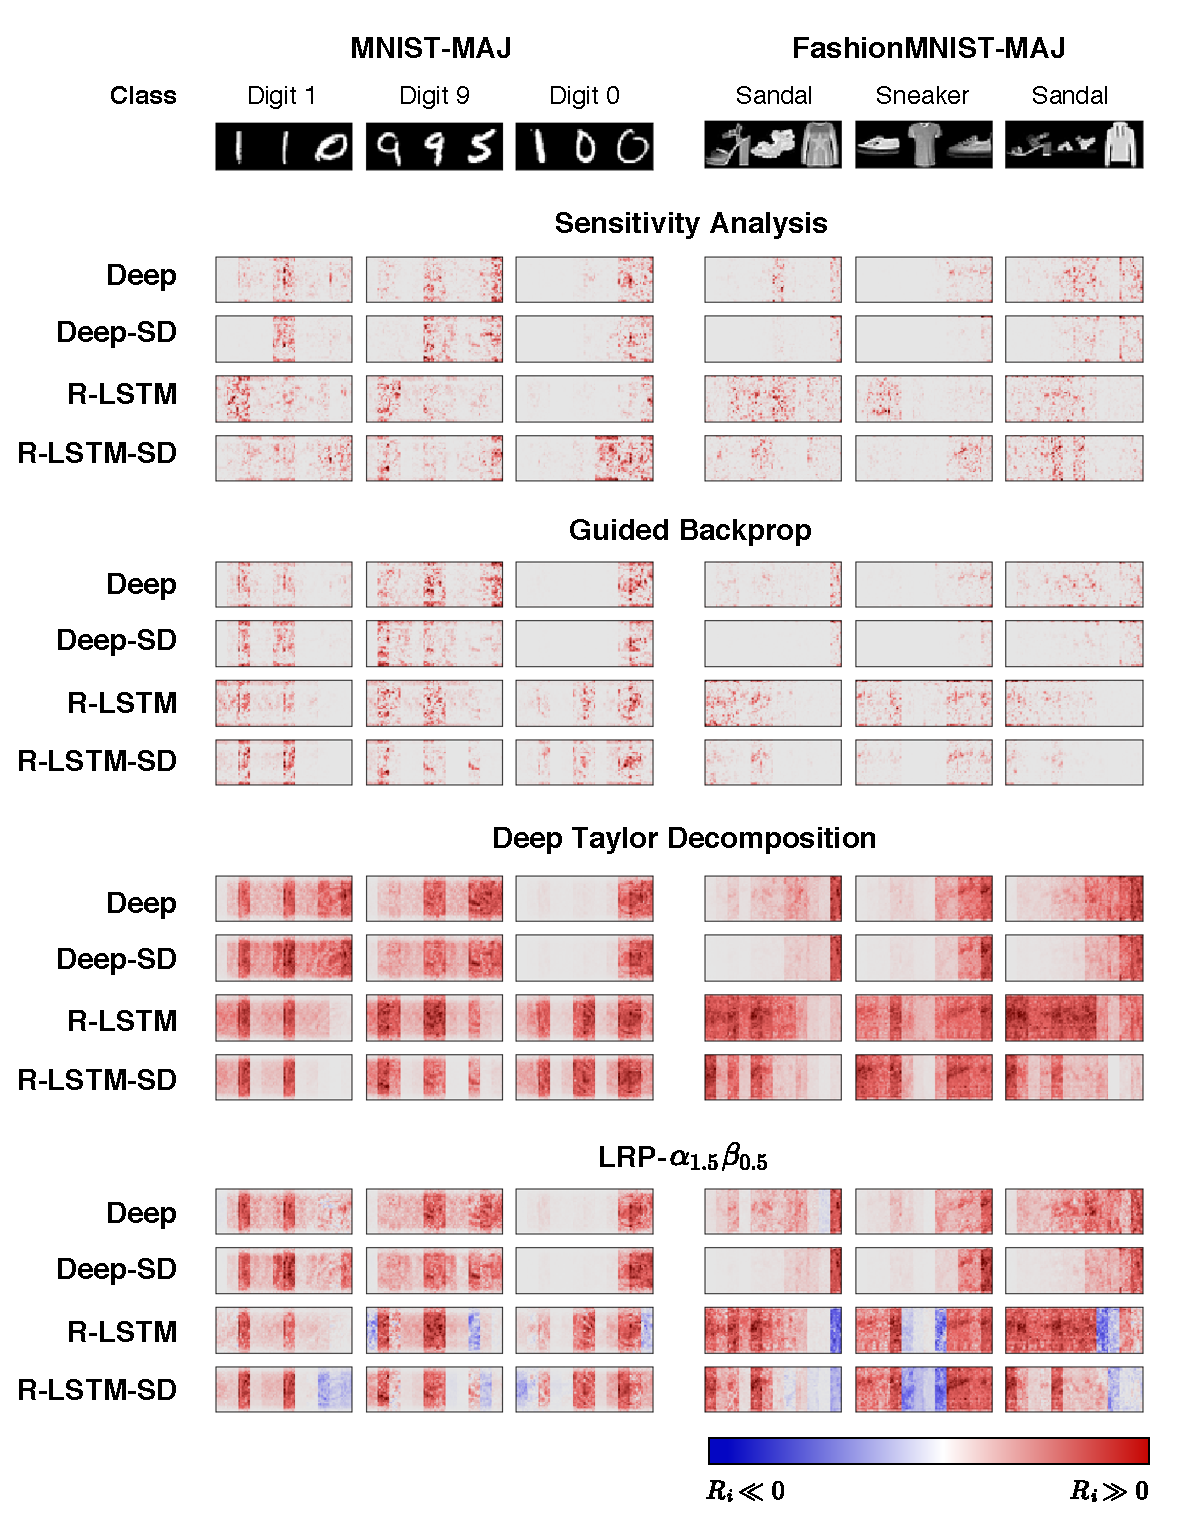
\includegraphics[width=\textwidth]{sketch/heatmap_msc_rlstm_exp}
\caption{..} 
\label{fig:heatmap_msc_rlstm_exp}
\end{figure}

\addfigure{\ref{fig:heatmap_msc_rlstm_exp}} shows results of the first part of this experiment. Here, variants of Deep and R-LSTM are compared. From the figure, it is obvious that R-LSTM gives better results than the Deep architecture. More precisely, we can directly observe the improvements from GB, DTD and $\lrpp$ heatmaps. Moreover, training with stationary dropout seems to produce R-LSTM with higher explanation capability. This is well notable on explanations from  DTD and $\lrpp$. In contrast, stationary dropout does not seem to have any prominent impact on the Deep architecture.


 \begin{figure}[!htb]
\centering
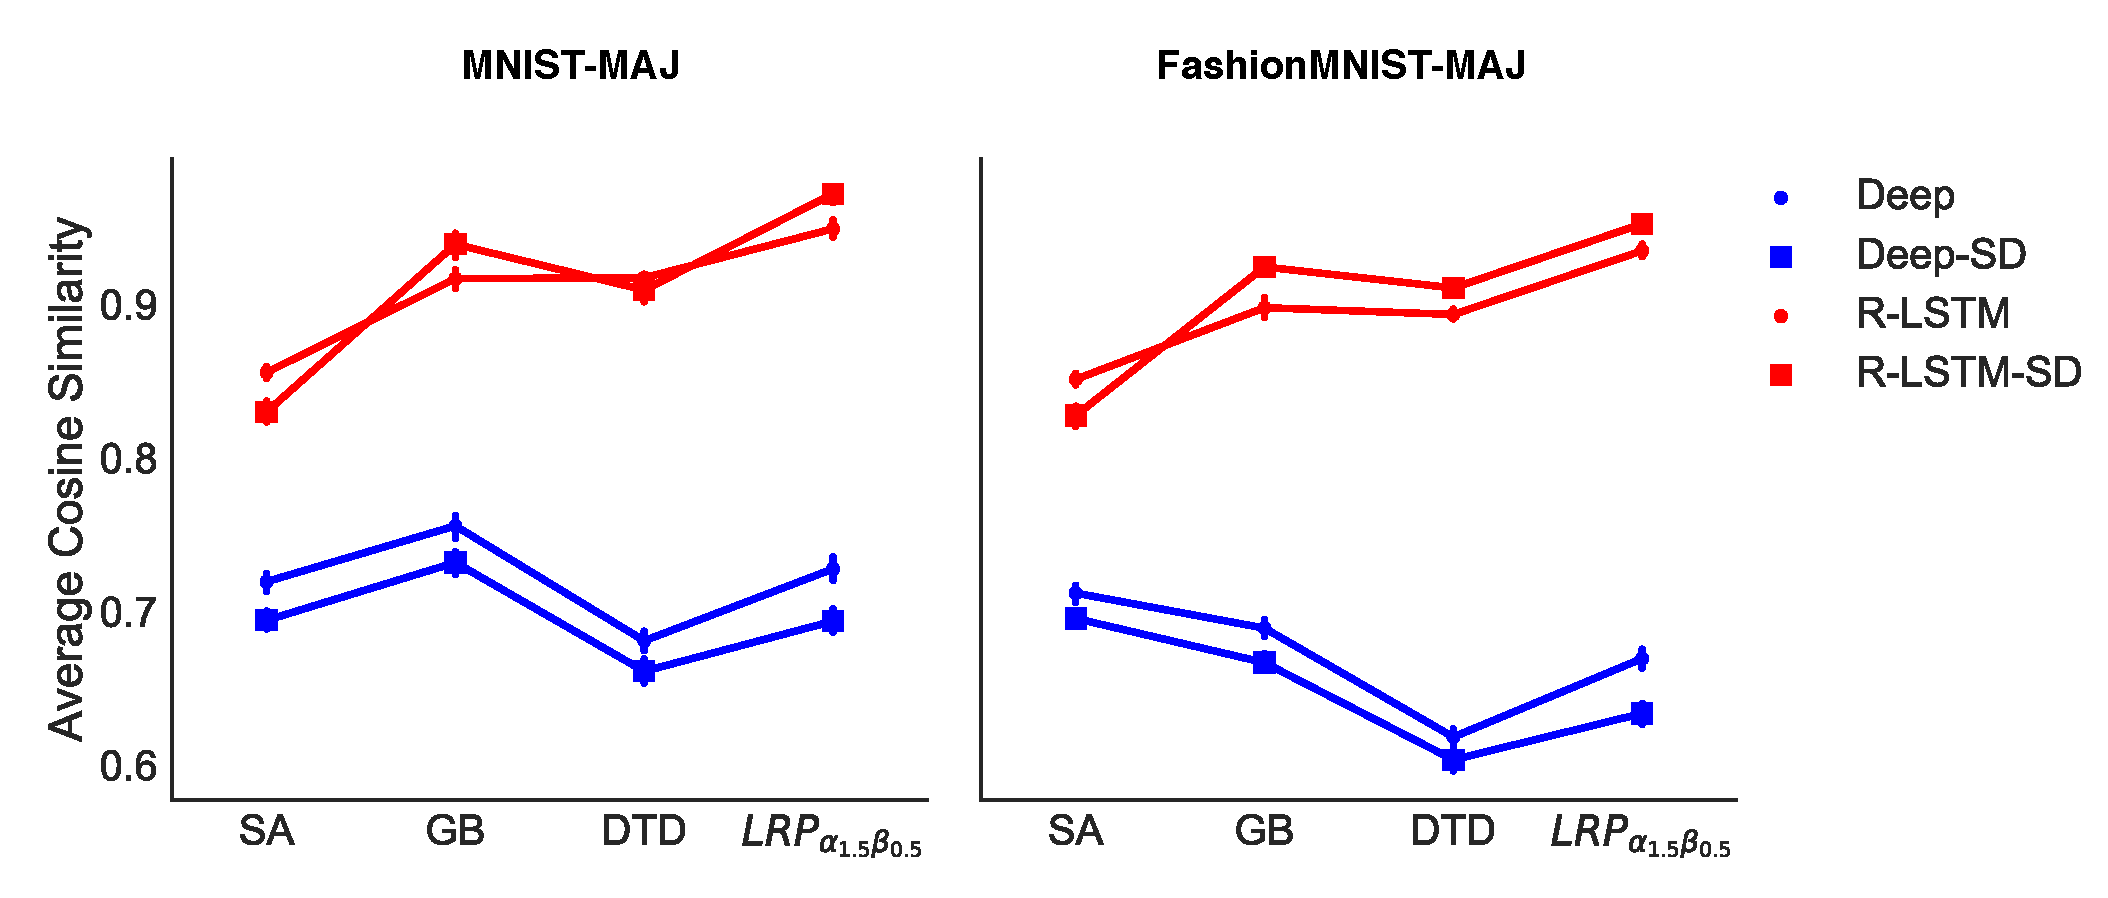
\includegraphics[width=\textwidth]{sketch/rel_dist_rlstm_exp}
\caption{..} 
\label{fig:rel_dist_rlstm_exp}
\end{figure}

\addfigure{\ref{fig:rel_dist_rlstm_exp}} presents the quantitative evaluation. As a reminder, these plots are averaged over models trained with cross validation procedure described in  Section \ref{sec:evaluation_med}. The figure shows that R-LSTM significantly improves relevance distribution than the Deep architecture regardless of explanation techniques.  This implies that decisions from R-LSTM can be better explained than the ones from the Deep architecture. Moreover, we can also see that the proportion of the improvement varies across methods. In particular, $\lrpp$ seems to have greater advantage from R-LSTM than the other methods.  

\addfigure{\ref{fig:rel_dist_rlstm_exp}}  also shows another interesting result where we can see that R-LSTM trained with stationary dropout, or R-LSTM-SD, performs much better than R-LSTM on FashionMNIST, while the two models have only slight difference on MNIST. This might be an effect from complexity of structures of FashionMNIST samples, as a result keeping dropout mask the same for all step would enable the network to efficiently learn latent features from homogenous input. In contrast, this does not seem to be the case for the Deep architecture. Particularly, we find that the percentage of Deep-SD is lower than Deep in any case.

 \begin{figure}[!htb]
\centering
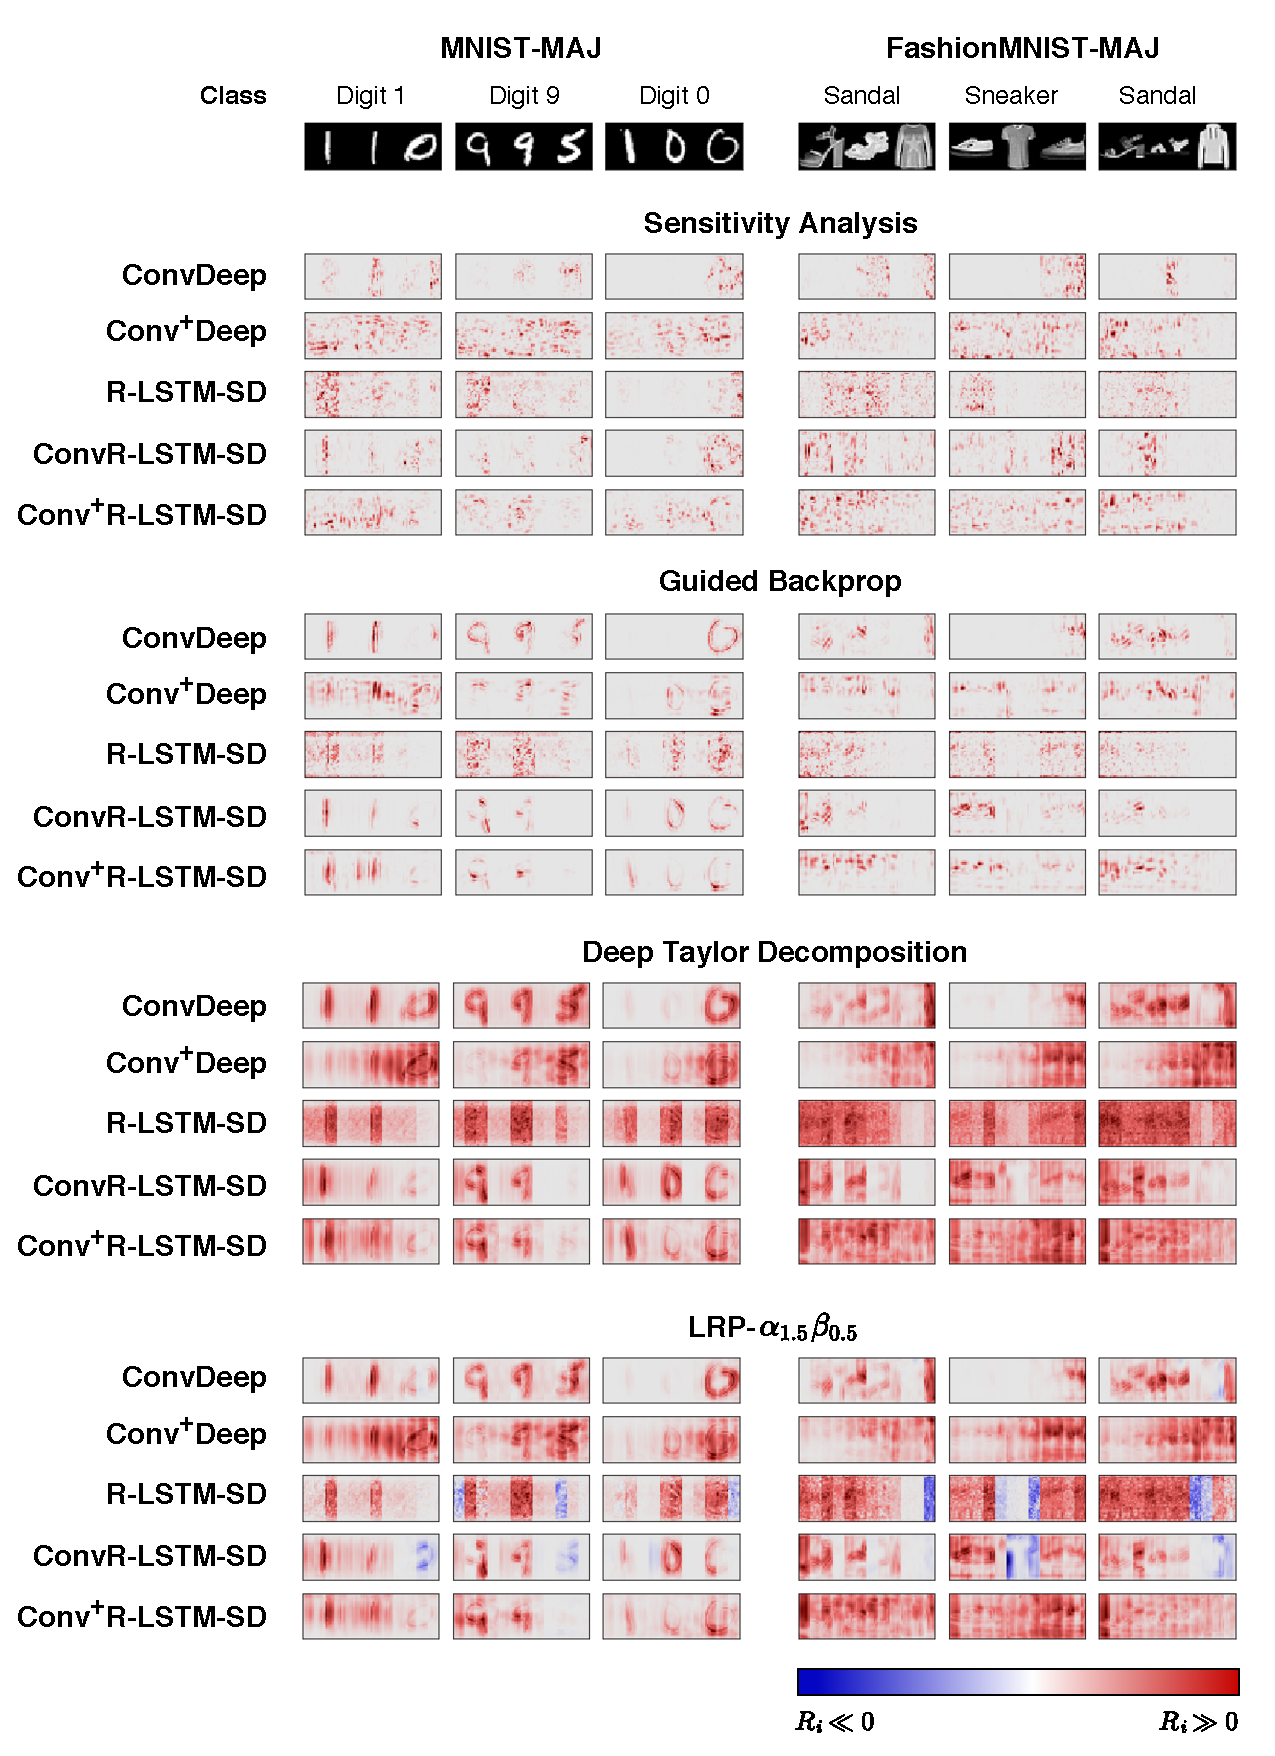
\includegraphics[width=\textwidth]{sketch/heatmap_msc_convtran_exp_v2}
\caption{..} 
\label{fig:heatmap_msc_convtran_exp}
\end{figure}
For the second part, we compare the ConvDeep architecture and the effect of literal connections as well as R-LSTM-SD with convolutional layers, ConvR-LSTM-SD. According to \addfigure{\ref{fig:heatmap_msc_convtran_exp}}, Conv$^+$Deep produces more diffuse heatmaps than ConvDeep. This is specially notable on heatmaps from SA  and GB method. Similarly, Conv$^+$Deep also produces worse results for DTD and $\lrpp$, for example consider Digit 1 and Digit 9.

\addfigure{\ref{fig:heatmap_msc_convtran_exp}} also shows relevance heatmaps from R-LSTM-SD equipped with convolutional and pooling layers, named ConvR-LSTM-SD, instead of a fully-connected layer. Comparing to R-LSTM-SD, having convolutional and pooling layers does improve  the quality of the heatmaps further. In particular, we can clearly see samples' structures from the results.

 \begin{figure}[!htb]
\centering
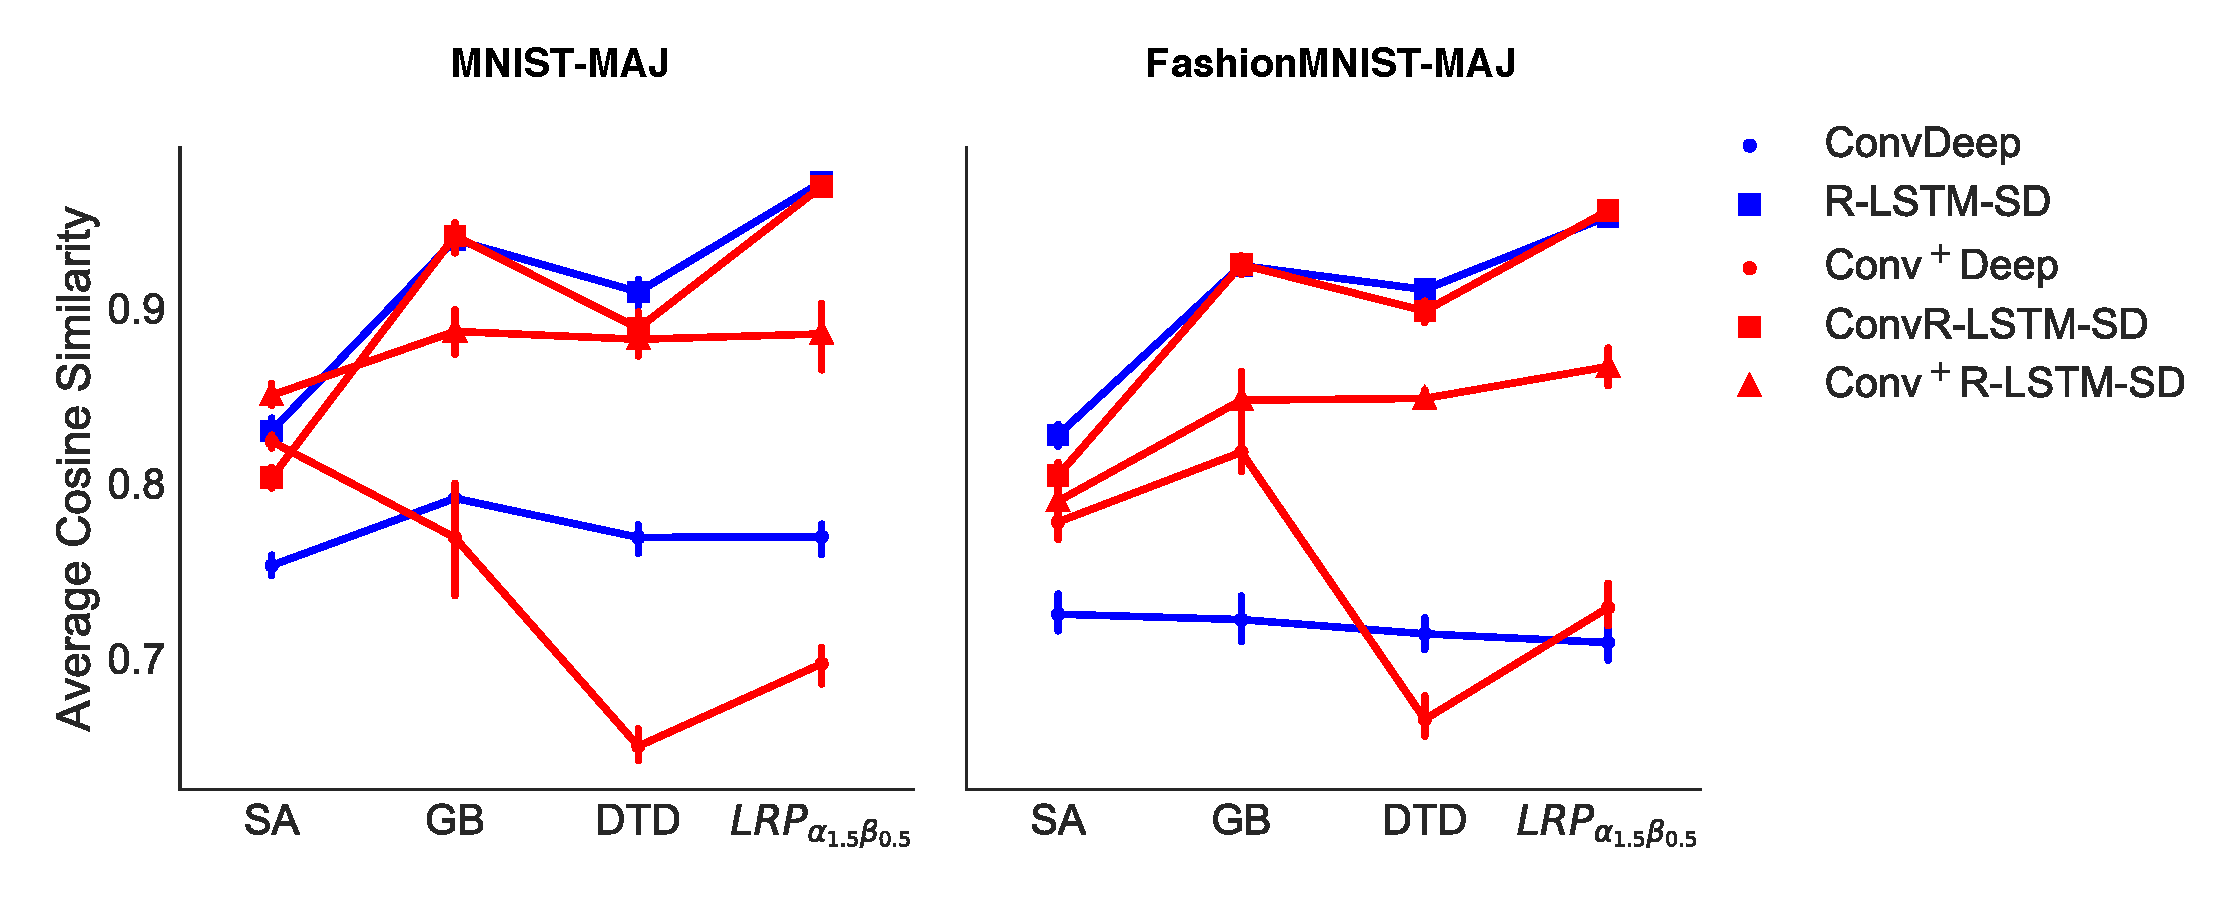
\includegraphics[width=\textwidth]{sketch/rel_dist_convdeep_trans_exp}
\caption{..} 
\label{fig:rel_dist_convdeep_trans_exp}
\end{figure}

\addfigure{\ref{fig:rel_dist_convdeep_trans_exp}} presents the quantitive result for the second part of the experiment. Here, ConvDeep and R-LSTM-SD are results from the previous experiments and used as baseline. Unexpectedly, literal connections considerably reduce the explanation capability of the ConvDeep architecture. For ConvR-LSTM-SD, its improvement seems to be only small fraction from R-LSTM-SD. In fact, using Tukey HSD test shows that the improvement is not statistically significant.



\subsection{Summary}
... \todo{writing summary}